\documentclass{article}
\usepackage[margin=1in]{geometry}
\usepackage{microtype}
\usepackage{setspace}
\usepackage{amsmath}
\usepackage{parskip}
\usepackage{amssymb}
\usepackage{graphicx}

\graphicspath{{../public/}}

\parskip=4ex
\date{}
\author{}

\title{5.1 Eigenvectors and Eigenvalues}

\begin{document}
  \maketitle
  \textbf{Introduction}\\
  Although a transformation $ x \mapsto Ax $ may move vectors in various directions, it often happens that there are special vectors on which the action of $ A $ is very simple

  \textbf{Ex 1}\\
  Let $ A=\begin{bmatrix}
      3 &-2\\
      1 &0
  \end{bmatrix}, u=
  \begin{bmatrix}
      -1\\
      1
  \end{bmatrix},
  v=\begin{bmatrix}
      2\\
      1
  \end{bmatrix} $. The images of $ u ~\&~ v $ under multiplication by $ A $ is shown in the figure below. It turns out that $ Av=2v $, so $ A $ "stretches" or dilates $ v $.
  \begin{center}
      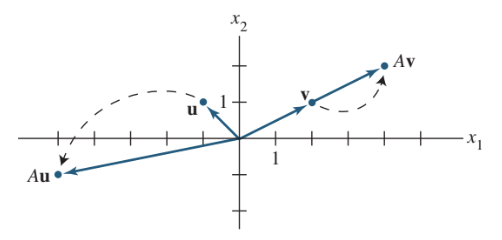
\includegraphics[width=6cm]{5_1_1}
  \end{center}

  \textbf{Definition}\\
  An eigenvector of an $ n \times n $ matrix $ A $ is a nonzero vector $ x $ such that $ Ax=\lambda x $ for some scalar $ \lambda $. A scalar $ \lambda $ is known as an eigenvalue of $ A $ if $ x $ is a nontrivial solution of $ Ax=\lambda x $. Such an $ x $ is called an eigenvector corresponding to $ \lambda $.

  \textbf{Ex 2}\\
  Let $ A=\begin{bmatrix}
      1 &6\\
      5 &2
    \end{bmatrix}, u=\begin{bmatrix}
      6\\
      -5
  \end{bmatrix}, ~\&~ v=\begin{bmatrix}
      3\\
      -2
  \end{bmatrix} $. Are $ u ~\&~ $ eigenvectors of $ A $.
  \[
      \begin{gathered}
      Au=\begin{bmatrix}
          1 &6\\
          5 &2
      \end{bmatrix}
      \begin{bmatrix}
          6\\
          -5
      \end{bmatrix}=\begin{bmatrix}
          -24\\
          20
      \end{bmatrix}=-4\begin{bmatrix}
          6\\
          -5
      \end{bmatrix}=-4u\\
      Av=\begin{bmatrix}
          1 &6\\
          5 &2
      \end{bmatrix}
      \begin{bmatrix}
          3\\
          -2
      \end{bmatrix}=
      \begin{bmatrix}
          -9\\
          11
      \end{bmatrix}\neq
      \lambda \begin{bmatrix}
          3\\
          -2
      \end{bmatrix}
      \end{gathered}
  \]

  $ u $ is an eigenvector corresponding to an eigenvalue (-4), but $ v $ is not an eigenvector of $ A $, because $ Av $ is not a scalar of $ v $.

  \textbf{Ex 3}\\
  Show that $ 7 $ is an eigenvalue of matrix $ A $ in Example $ 2 $, and find the corresponding eigenvectors.
  \[
      Ax=7x
  \]
  
  The scalar $ 7 $ is an eigenvalue of $ A $ if and only if the equation has a nontrivial solution.
  \[
      \begin{gathered}
      Ax=7x\\
      Ax-7x=0\\
      (A-7)x=0\\
      (A-7I)x=0\\
      ~\\
      A-7I=
      \begin{bmatrix}
          1 &6\\
          5 &2
      \end{bmatrix}-
      \begin{bmatrix}
          7 &0\\
          0 &7
      \end{bmatrix}=
      \begin{bmatrix}
          -6 &6\\
          5 &-5
      \end{bmatrix}\\
      ~\\
      \begin{bmatrix}
          -6 &6\\
          5 &-5
      \end{bmatrix}
      \begin{bmatrix}
          x_{1}\\
          x_{2}  
      \end{bmatrix}=
      \begin{bmatrix}
          0\\
          0
      \end{bmatrix}\\
      \begin{bmatrix}
          -6 &6 &0\\
          5 &-5 &0
      \end{bmatrix}\to
      \begin{bmatrix}
          1 &-1 &0\\              
          0 &0 &0
      \end{bmatrix} 
      \end{gathered}
  \]

  The columns of $ A-7I $ are linearly dependent so $ A-7I $ has nontrivial solutions. The general solution has the form $ x_{2} \begin{bmatrix}
          1\\
          1
  \end{bmatrix} $. Each vector of this form with a nonzero $ x_{2} $ is an eigenvector corresponding to $ \lambda=7 $.

  Do note that that although row reduction can be used to find eigenvectors, it cannot be used to find eigenvalues.

 $ \lambda $ is an eigenvalue of an $ n \times n $ matrix $ A $ if and only if the equation
 \[
   (A-\lambda I)x=0
 \]

 has a nontrivial solution. The null space of $ A-\lambda I $  of $ (A-\lambda I)x=0$ is the set of all solutions to $ (A-\lambda I)x=0 $. So the set is a subspace of $ \mathbb{R}^{n} $ and is called the eigenspace of $ A $ corresponding to $ \lambda $. Meaning the eigenspace consists of the zero vector and all the eigenjvectors corresponding to $ \lambda $.

 \textbf{Ex 4}\\
 Let $ A=\begin{bmatrix}
     4 &-1 &6\\
     2 &1 &6\\
     2 &-1 &8
 \end{bmatrix} $. An eigenvalue of $ A $ is 2. Find a basis for the corresponding eigenspace.
 \[
     \begin{gathered}
     A-2I = \begin{bmatrix}
         4 &-1 &6\\
         2 &1 &6\\
         2 &-1 &8
     \end{bmatrix}-
     \begin{bmatrix}
         2 &0 &0\\
         0 &2 &0\\
         0 &0 &2
     \end{bmatrix}=
     \begin{bmatrix}
        2 &01 &6\\
        2 &01 &6\\
        2 &01 &6
     \end{bmatrix}\\
     ~\\
     \begin{bmatrix}
         2 &-1 &6 &0\\
         2 &-1 &6 &0\\
         2 &-1 &6 &0
     \end{bmatrix} \to
     \begin{bmatrix}
         2 &-1 &6 &0\\
         0 &0 &0 &0\\
         0 &0 &0 &0
     \end{bmatrix}
     \end{gathered}
 \]

 $ (A-2I)x=0 $ has free variables, so $ 2 $ is indeed an eigenvalue of $ A $. The general solution is
 \[
   \begin{bmatrix}
       x_1\\
       x_2\\
       x_3
   \end{bmatrix}=
   x_2\begin{bmatrix}
       \frac{1}{2} \\
       1\\
       0
   \end{bmatrix} +
   x_3\begin{bmatrix}
       -3\\
       0\\
       1
   \end{bmatrix}
 \]

 So the basis is
 \[
   \text{\large{\{}} \begin{bmatrix}
       1\\
       2\\
       0
   \end{bmatrix},
   \begin{bmatrix}
       -3\\
       0\\
       1
   \end{bmatrix}
 \text{\large{\}}}
 \]
 
 


 


  

\end{document}
